\section{Methods and Implementation}\label{methods and implementation}

This section presents different processing techniques with the aim of solving the task at hand. SEALAB's current solutions is explained and discussed. The new implementation is explained step by step followed by images showing the process and the results.


\subsection{Previous implementation done by SEALAB}

{\color{red}
Write about what they have already tried out. 
they have tried interpolation filling out the fish. Show picture of the green fish. 
This did work, but the interpolation algorithm take forever to run and you can see the colors that represent the depth of the fish is not that even.

What is also now done is get the p-data directly from the Raytrix software, then make a depthmap from the p-data and use the p-data in the volume algorithm. What I want to do is get the depthmap directly from the Raytrix, do some work on it, extract the p-data based on color, then send the data to through the volume algorithm. 
}

%%%%%%%%%%%%%%%%%%%%%%%%%%%%%%%%%%%%%%%%%%%%%%%%%%%%%%%%%%%%%%%%%%%%%%


\subsection{Depthmap enhancement} \label{section:depthmap}

\subsubsection{Morphological Closing and Object Detection}

The approach used to better the depthmap image used morphological closing on the depthmap to even out the color and fill the holes. It started with color-filtering to remove particles too close or too far behind the main object. The algorithm also found the largest contour from the original image to use as a mask. The algorithm followed the steps below. The complete code can be found in section \ref{code}.
\begin{enumerate}
    \item \textbf{Filter out unwanted colors:}
    Color-filtering was done by looping through each pixel in the image and setting it to black if its blue-value was too high, green-value too low or red-value too low. This removed all particles in the image that was too close or to far behind. 
    \item \textbf{Remove small particles:}
    Removal of small particles was done by eroding twice followed by dilating twice. Further removal would remove to much of the fish.
    \item \textbf{Find largest contour:}
    Finding the largest contour followed these steps: \cite{website:largest_contour_code_explanation}
    \begin{enumerate}[label*=\arabic*.]
        \item Convert to grayscale and normalize
        \item Sobel edge detector
        \item Dilate
        \item Floodfill
        \item Erode
        \item Find largest contour
    \end{enumerate}
    The resulting images is shown in figure \ref{fig:find_largest_contour}.
    \item \textbf{Morphological closing on color-filtered image:}
    To fill out the holes in the fish in an even and fast way, morphological closing was used.
    \item \textbf{Mask the morphological closed image with the largest contour:}
    Because the morphological closing operations would expand the fish, the largest contour was used as a mask to gain the final result. 
\end{enumerate}

Figure \ref{fig:algorithm} shows the steps done by the algorithm.

The algorithm was tested on different depthmap images, and gave very good results on many of them. It was also tested to find the largest contour from the totalfocus image instead of the depthmap, but the depthmap returned a more accurate contour. Figure \ref{fig:algorithm_test} shows the results from 4 different depthmaps on the same fish.
The result is good compared to the original depthmap, but the depthmap computed from the Raytrix software could be improved. This is most likely done by different lightning, or by giving the background a different color.
Painting the test facility black was tried, but it only resulted in missing spots on the fishes back instead of its bog.


\begin{figure}[H]
    \begin{subfigure}{0.48\textwidth}
        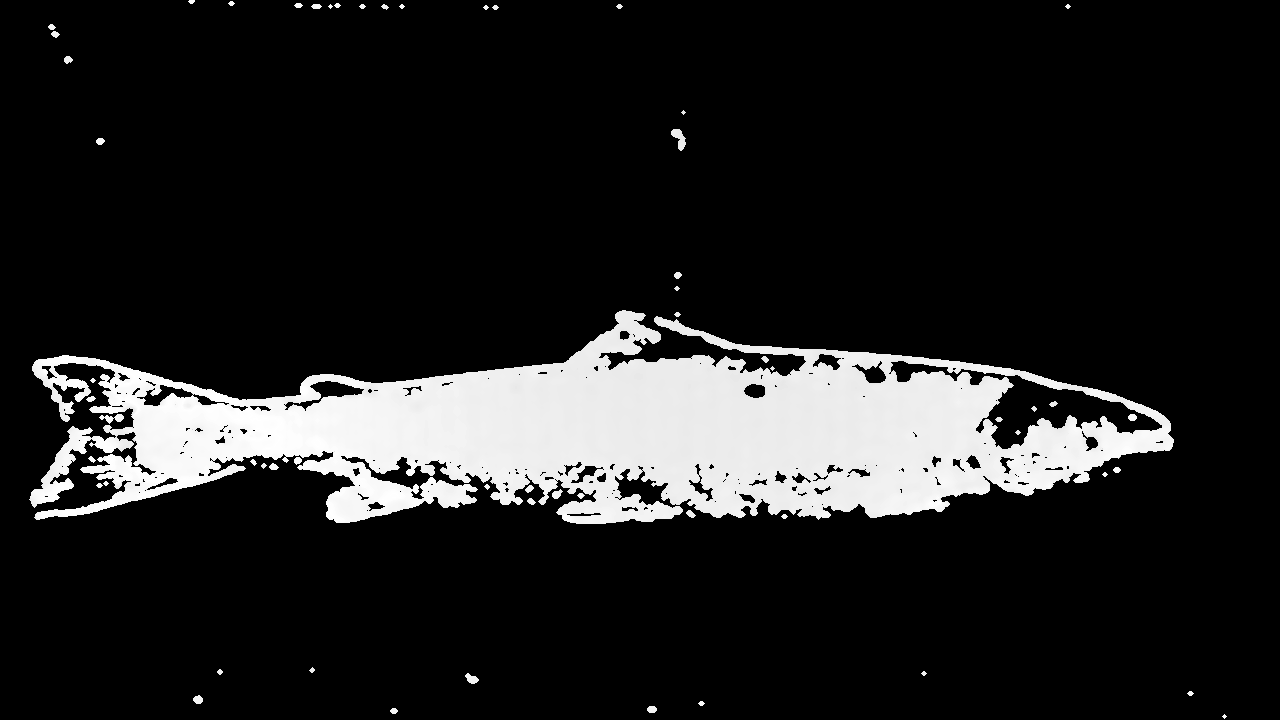
\includegraphics[width=\linewidth]{images/implementation/4_1_grayscale}
        \caption{Converted to grayscale} 
        \label{fig:grayscale}
    \end{subfigure}\hspace*{\fill}
    \begin{subfigure}{0.48\textwidth}
        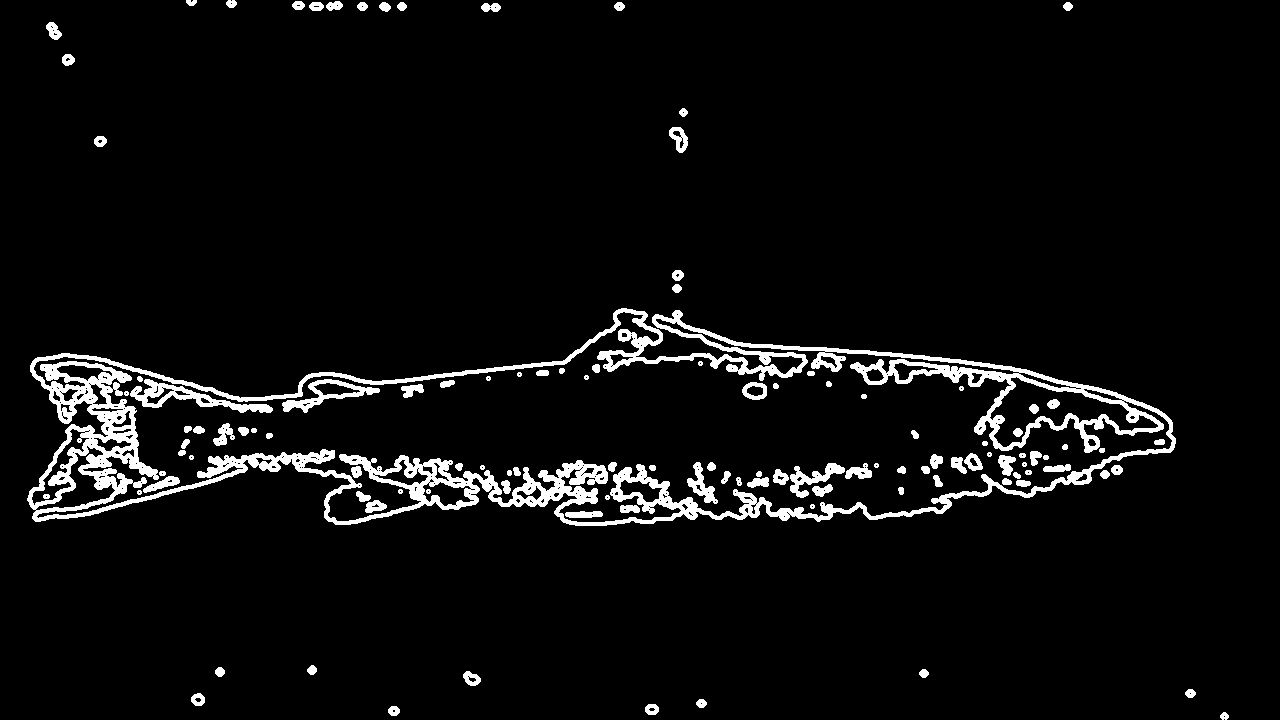
\includegraphics[width=\linewidth]{images/implementation/4_2_edge_detector}
        \caption{Edge detection} 
        \label{fig:edge_detection}
    \end{subfigure}
    
    \medskip
    \begin{subfigure}{0.48\textwidth}
        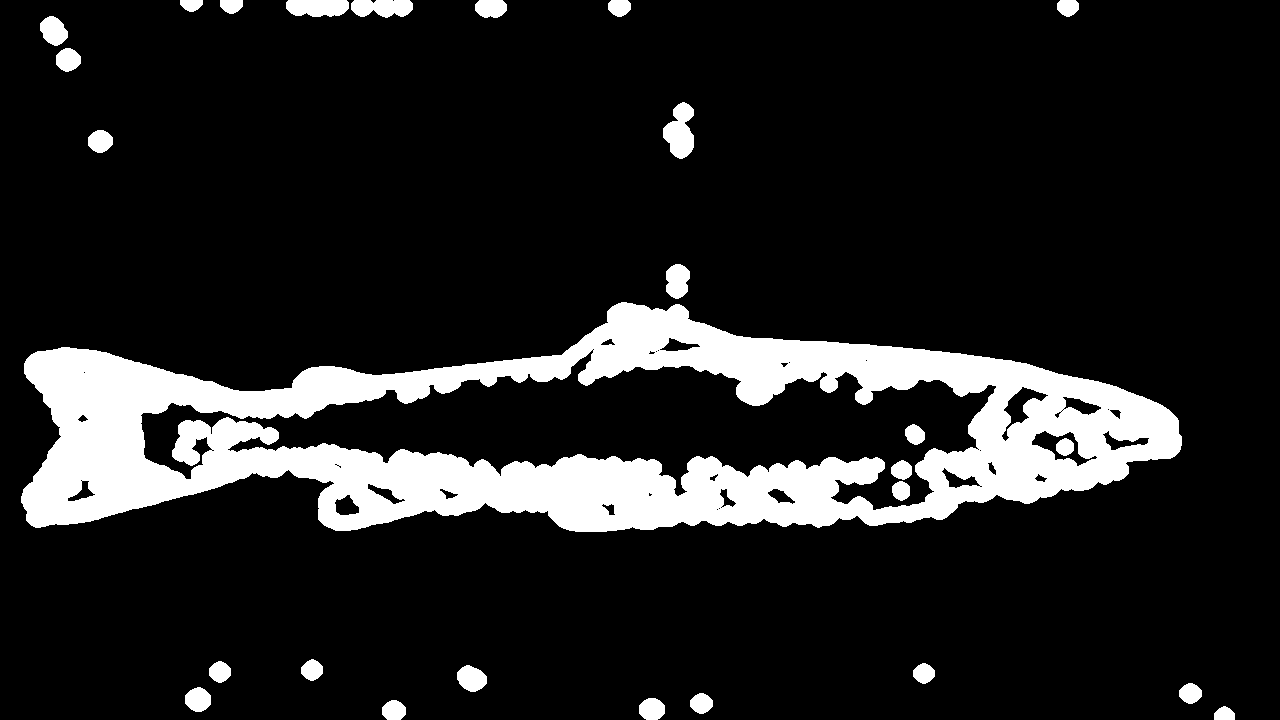
\includegraphics[width=\linewidth]{images/implementation/4_3_dilate}
        \caption{Dilate} 
        \label{fig:dilate_contour}
    \end{subfigure}\hspace*{\fill}
    \begin{subfigure}{0.48\textwidth}
        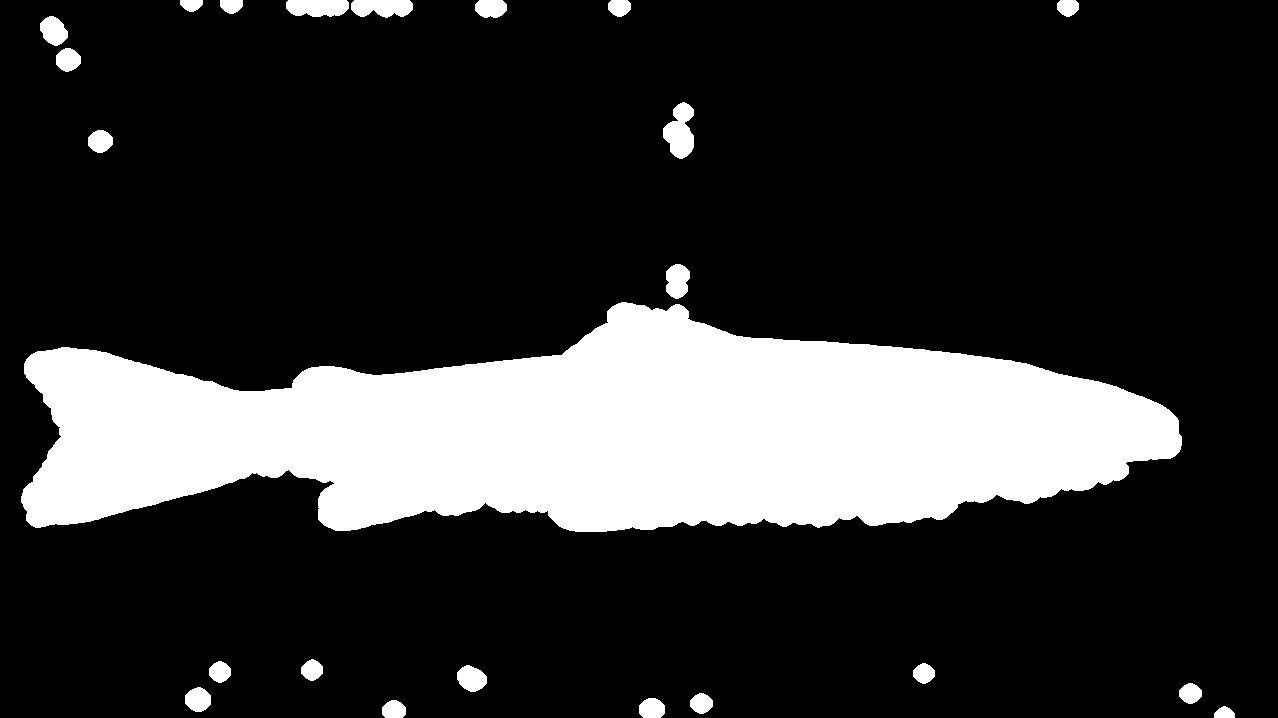
\includegraphics[width=\linewidth]{images/implementation/4_4_floodfill}
        \caption{Floodfill} 
        \label{fig:floodfill}
    \end{subfigure}
    
    \medskip
    \begin{subfigure}{0.48\textwidth}
        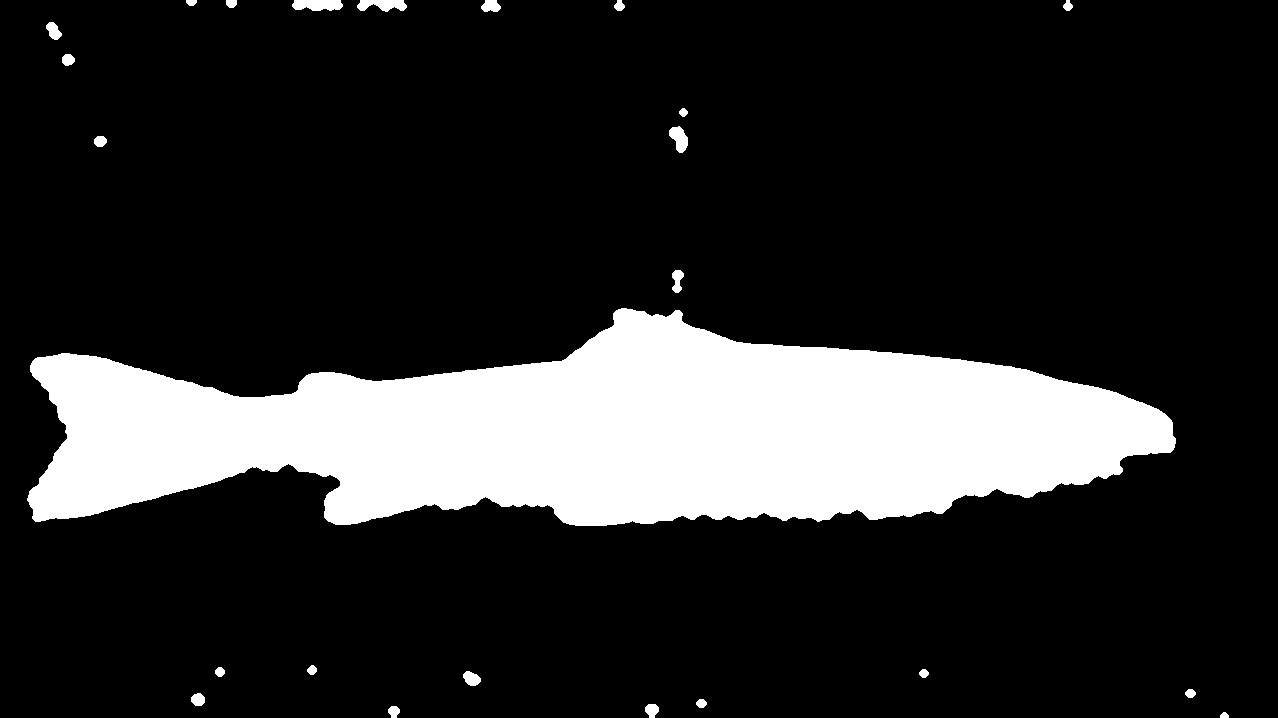
\includegraphics[width=\linewidth]{images/implementation/4_5_erode}
        \caption{Erode} 
        \label{fig:erode_contour}
    \end{subfigure}\hspace*{\fill}
    \begin{subfigure}{0.48\textwidth}
        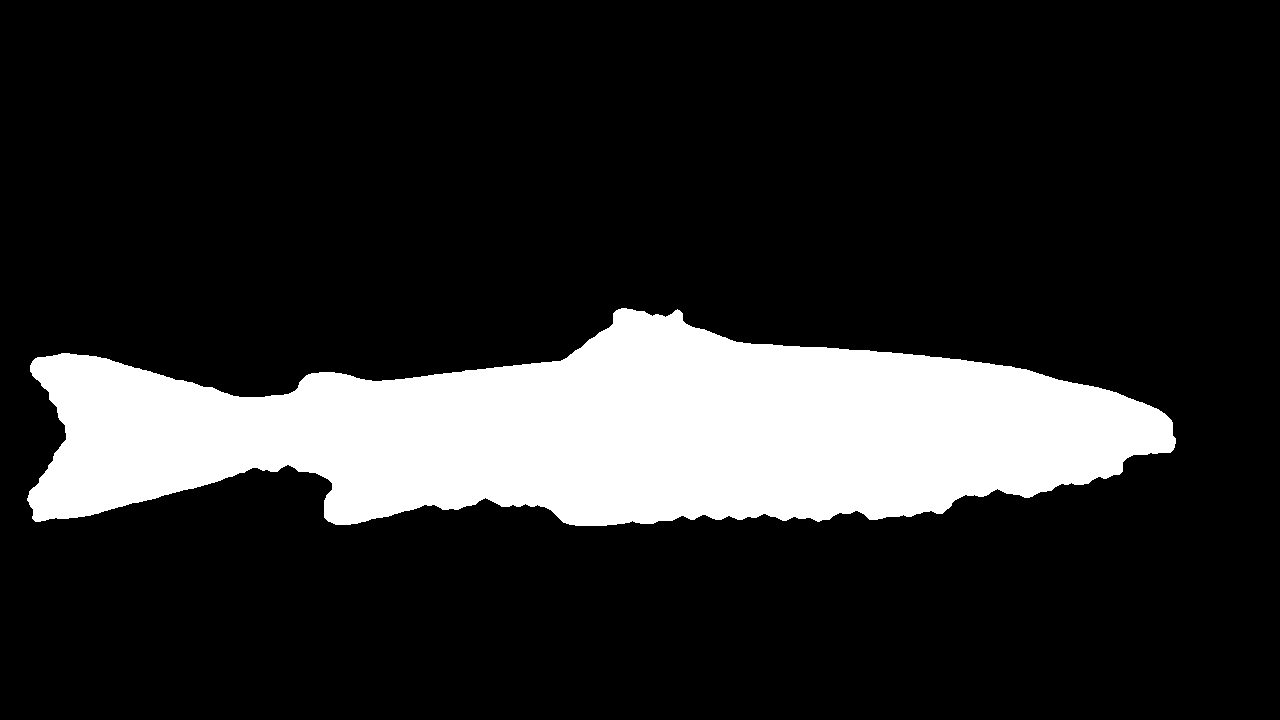
\includegraphics[width=\linewidth]{images/implementation/4_largest_contour}
        \caption{Largest contour} 
        \label{fig:largest_contour_2}
    \end{subfigure}
    \caption{Finding the largest contour} 
    \label{fig:find_largest_contour}
\end{figure}


\begin{figure}[H]
    \begin{subfigure}{0.48\textwidth}
        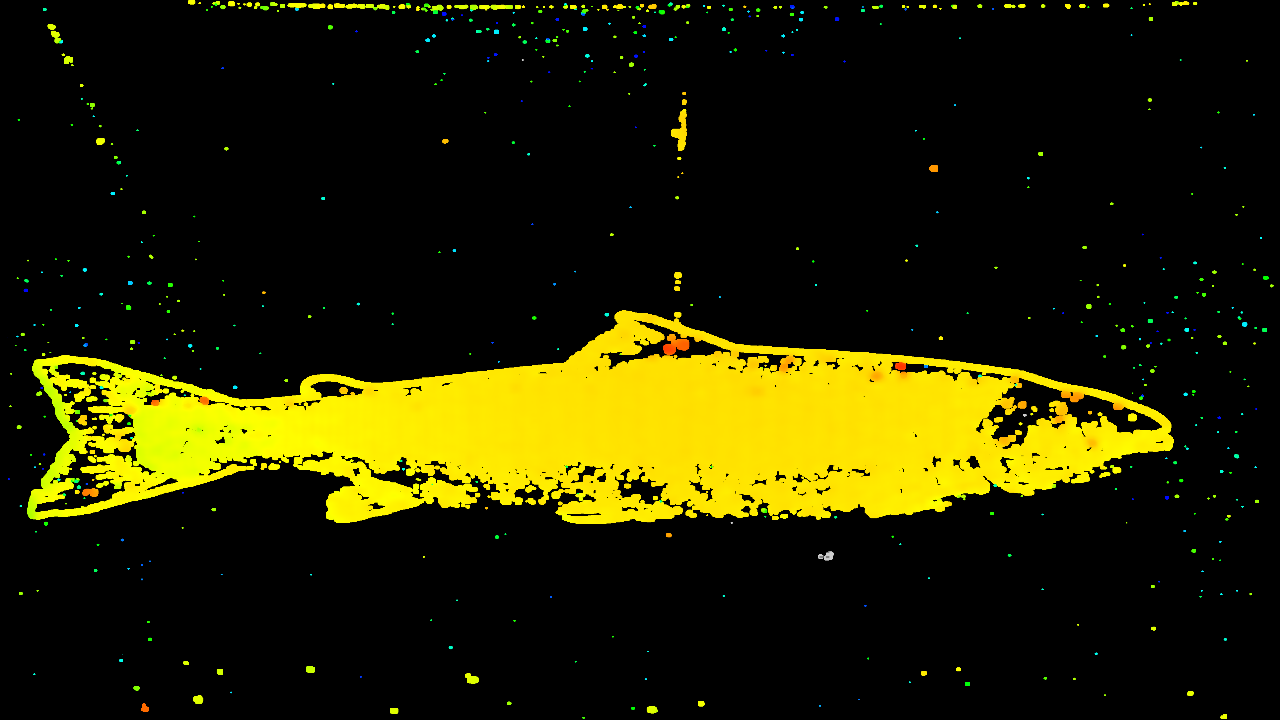
\includegraphics[width=\linewidth]{images/implementation/1_original}
        \caption{Original depthmap image} 
        \label{fig:original_depthmap}
    \end{subfigure}\hspace*{\fill}
    \begin{subfigure}{0.48\textwidth}
        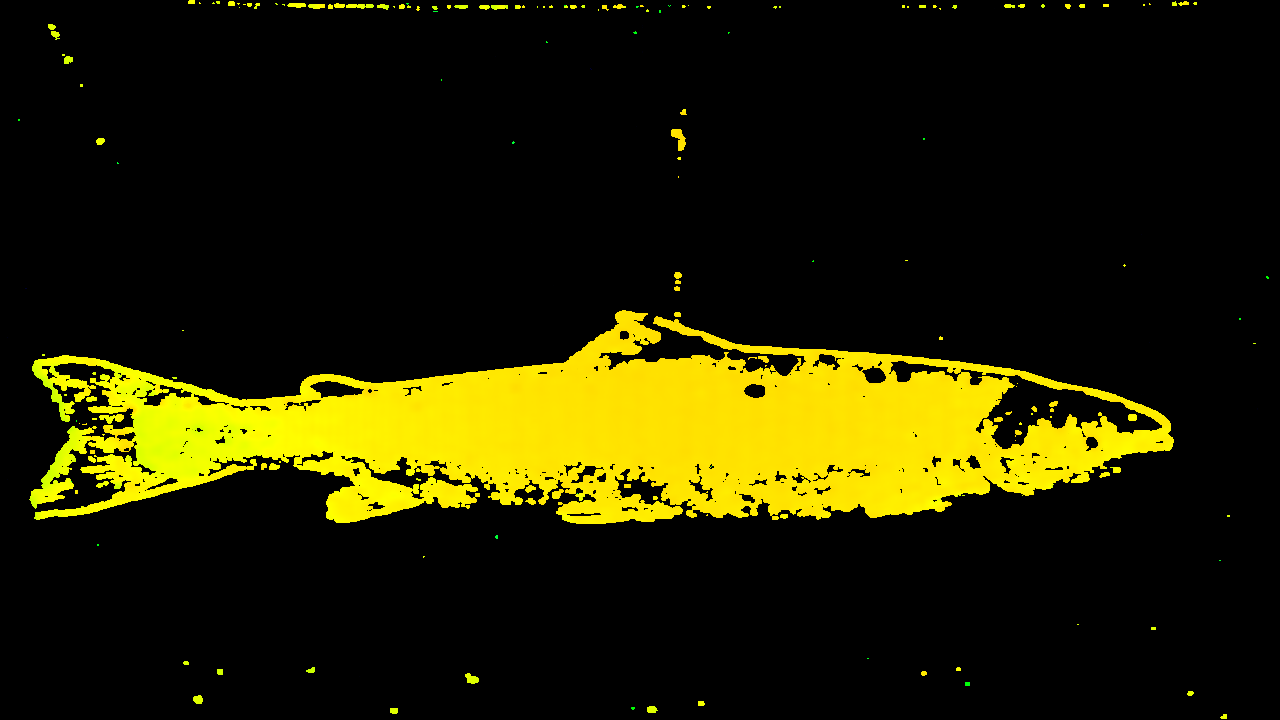
\includegraphics[width=\linewidth]{images/implementation/2_color_filtering}
        \caption{Color-filtered image} 
        \label{fig:color_filtering}
    \end{subfigure}
    
    \medskip
    \begin{subfigure}{0.48\textwidth}
        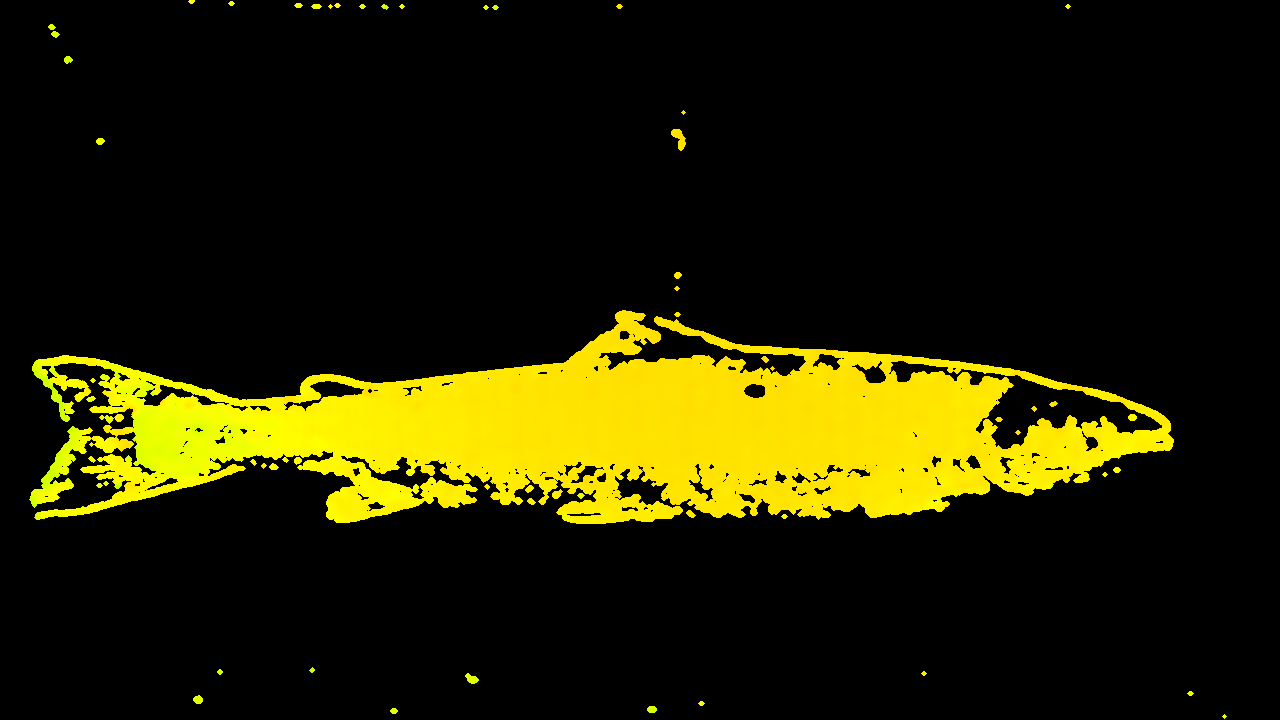
\includegraphics[width=\linewidth]{images/implementation/3_remove_particles}
        \caption{Removal of small particles} 
        \label{fig:remove_particles}
    \end{subfigure}\hspace*{\fill}
    \begin{subfigure}{0.48\textwidth}
        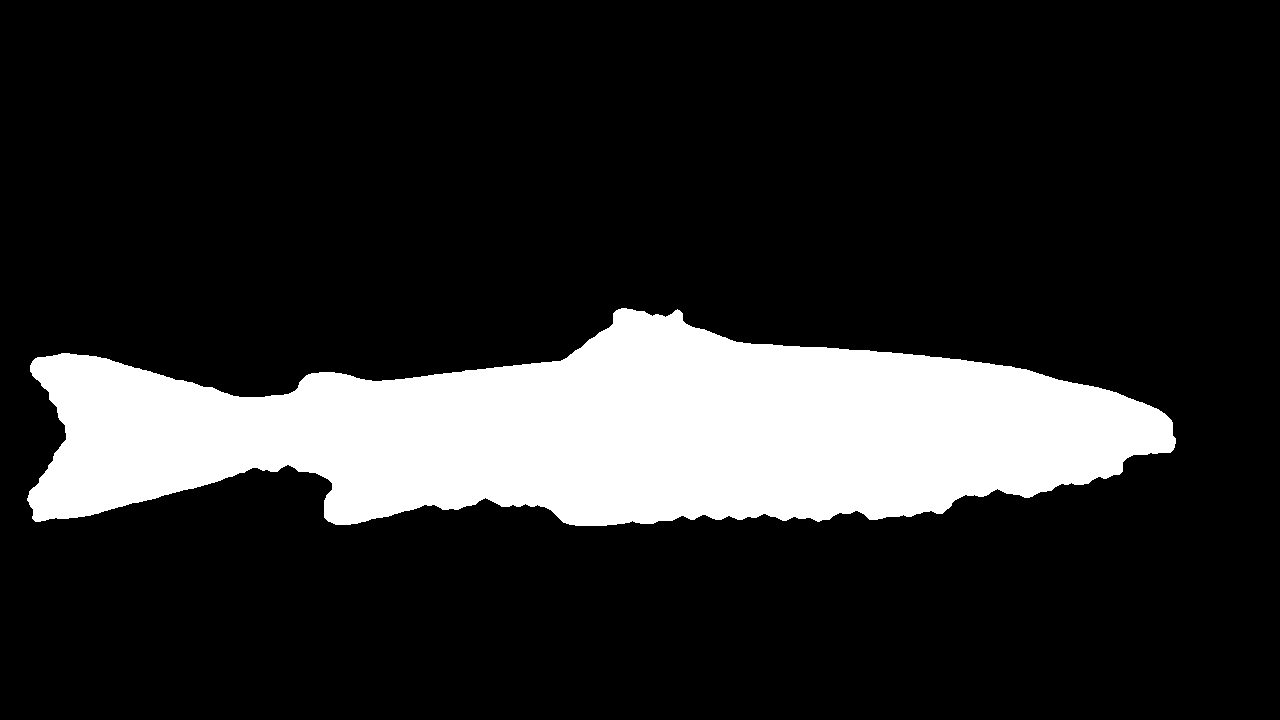
\includegraphics[width=\linewidth]{images/implementation/4_largest_contour}
        \caption{Largest contour} 
        \label{fig:largest_contour}
    \end{subfigure}
    
    \medskip
    \begin{subfigure}{0.48\textwidth}
        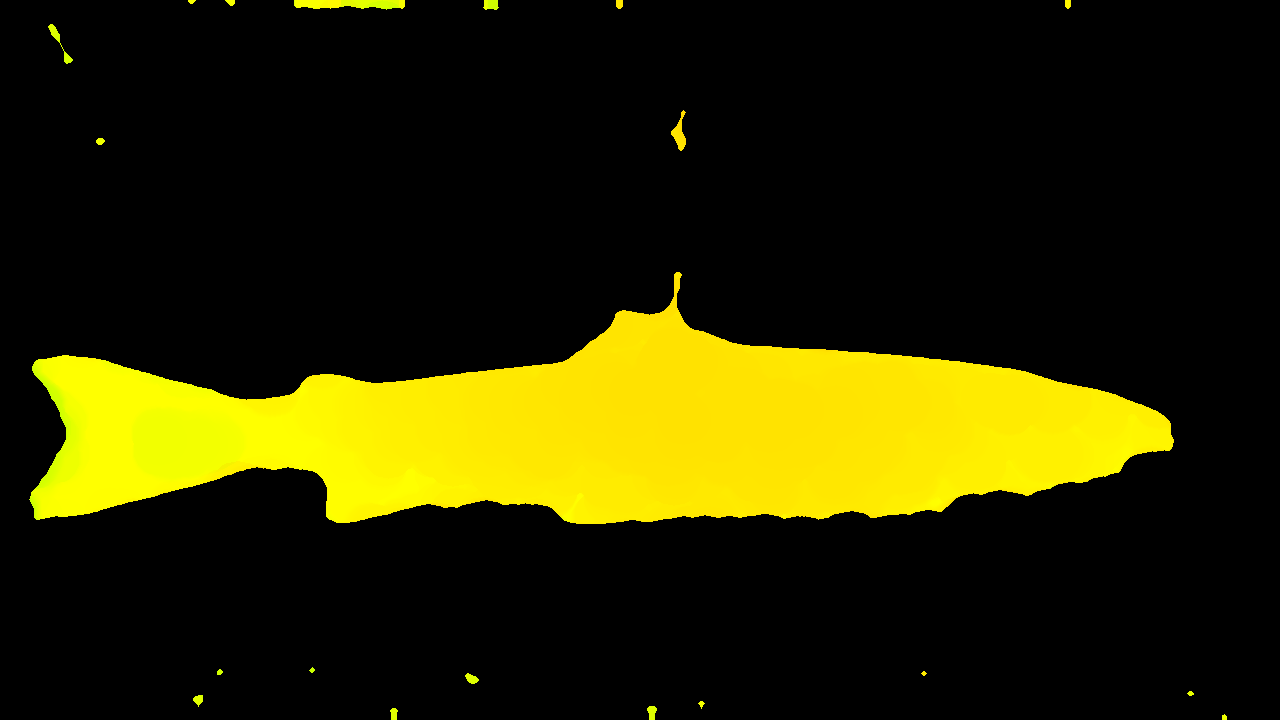
\includegraphics[width=\linewidth]{images/implementation/5_closing_on_color_filtered_image}
        \caption{Morphological closing} 
        \label{fig:morphological_closing}
    \end{subfigure}\hspace*{\fill}
    \begin{subfigure}{0.48\textwidth}
        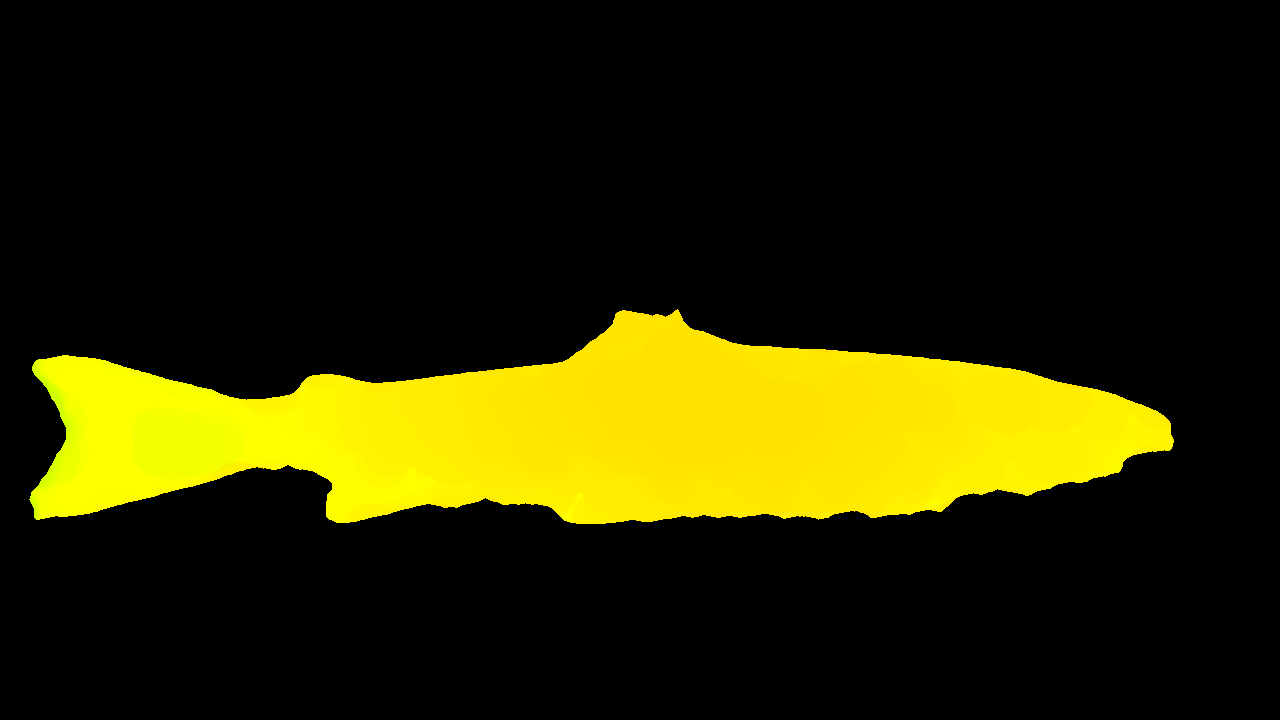
\includegraphics[width=\linewidth]{images/implementation/6_masked_source}
        \caption{Masked image} 
        \label{fig:masked_source}
    \end{subfigure}
    \caption{Morphological closing and masking with largest contour} 
    \label{fig:algorithm}
\end{figure}


\begin{figure}[H]
    \begin{subfigure}{0.48\textwidth}
        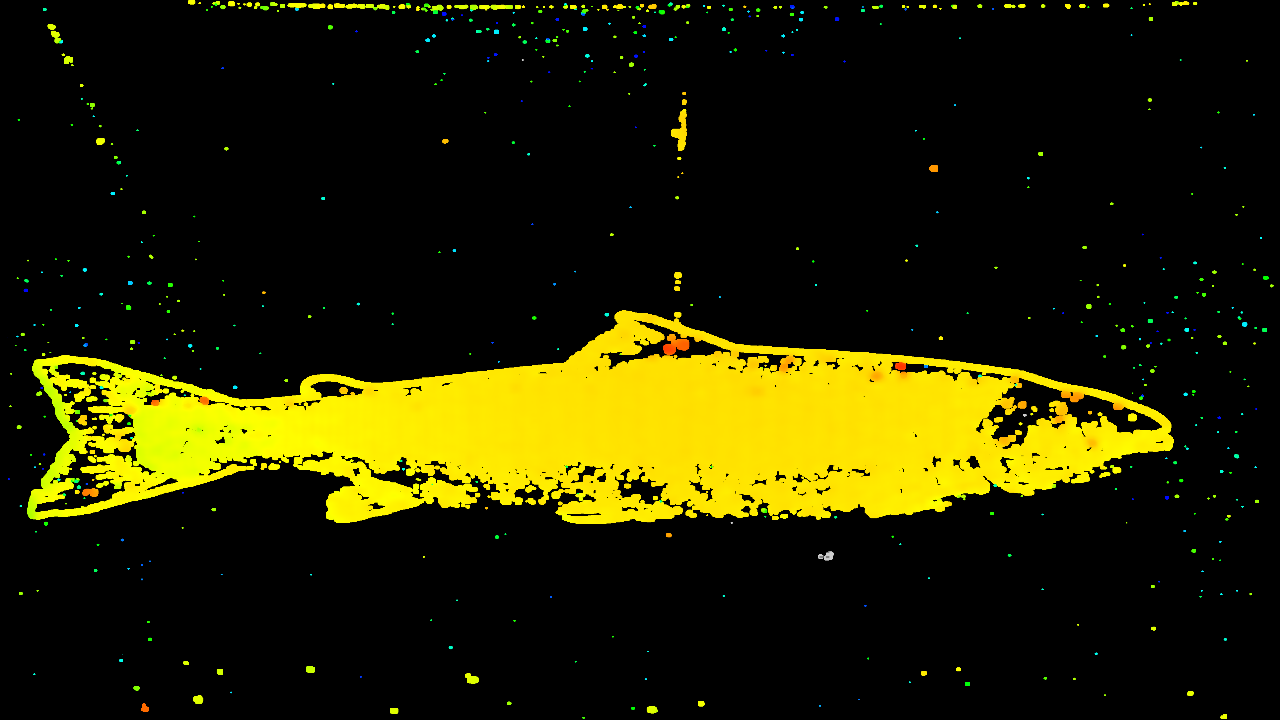
\includegraphics[width=\linewidth]{images/implementation/algorithm_test/original_63}
        \caption{Original depthmap image} 
        \label{fig:original_depthmap_63}
    \end{subfigure}\hspace*{\fill}
    \begin{subfigure}{0.48\textwidth}
        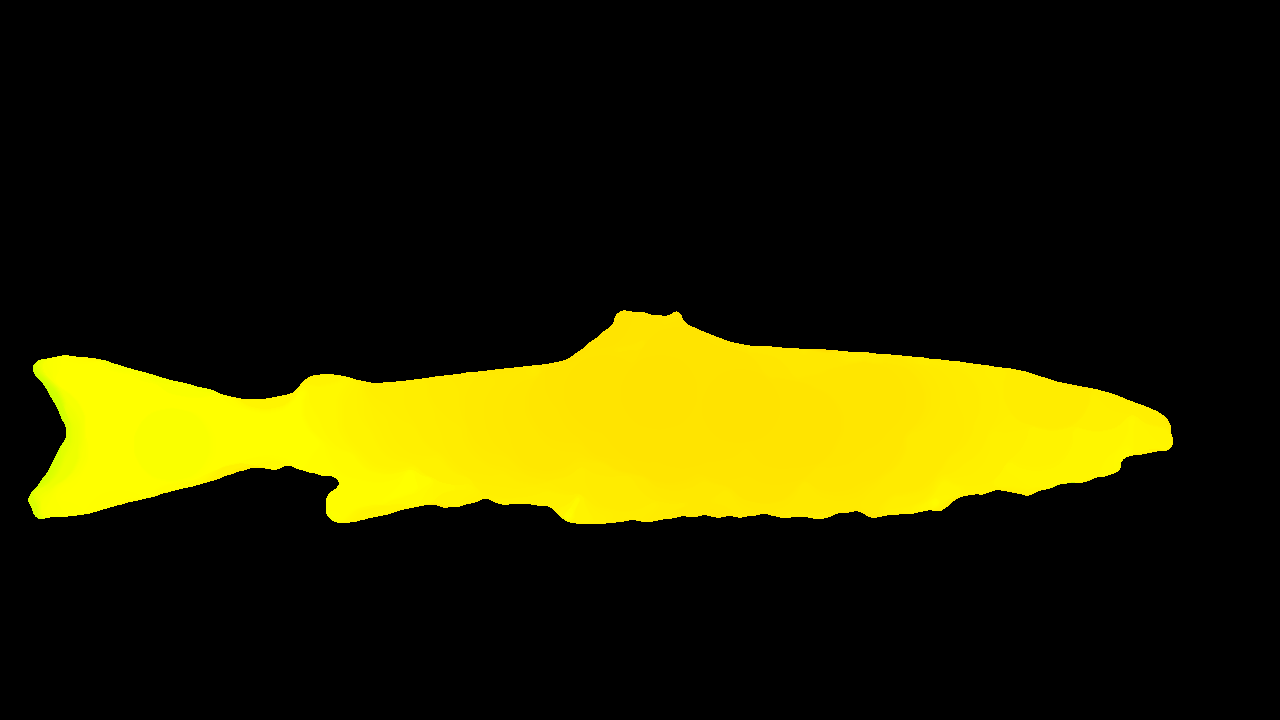
\includegraphics[width=\linewidth]{images/implementation/algorithm_test/median_filter_63}
        \caption{Result} 
        \label{fig:result_63}
    \end{subfigure}
    
    \medskip
    \begin{subfigure}{0.48\textwidth}
        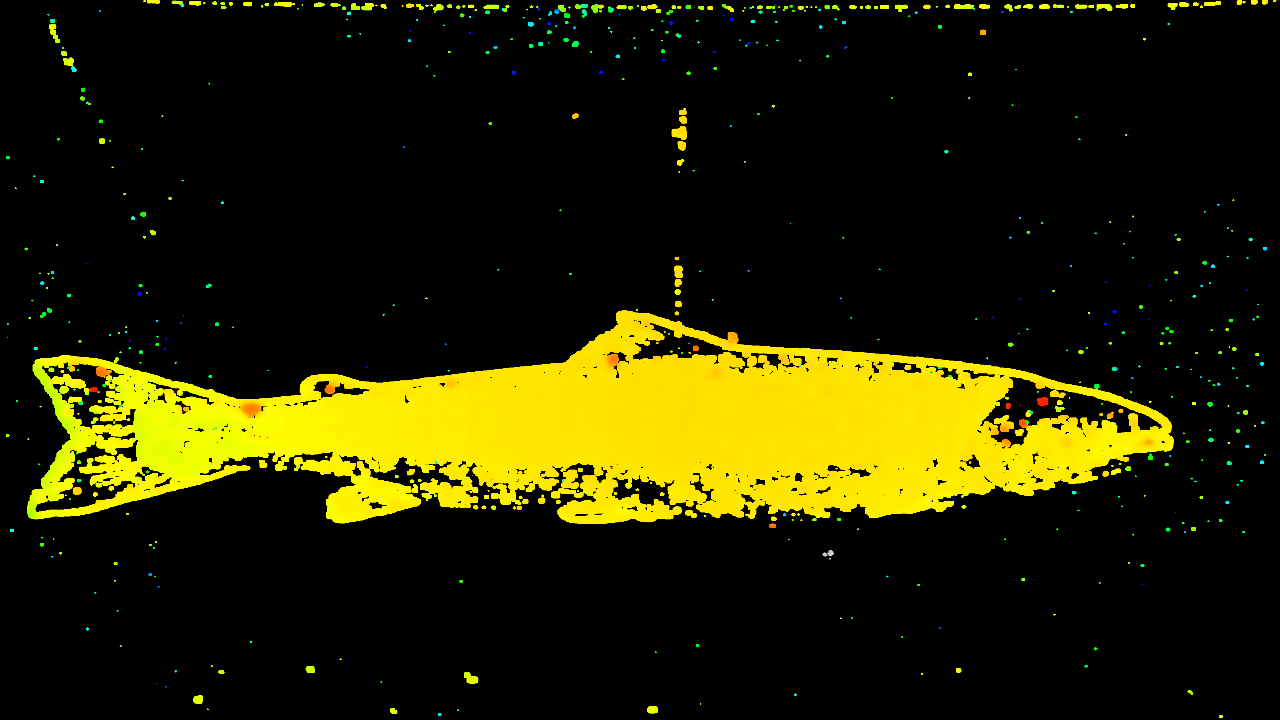
\includegraphics[width=\linewidth]{images/implementation/algorithm_test/original_73}
        \caption{Original depthmap image} 
        \label{fig:original_depthmap_73}
    \end{subfigure}\hspace*{\fill}
    \begin{subfigure}{0.48\textwidth}
        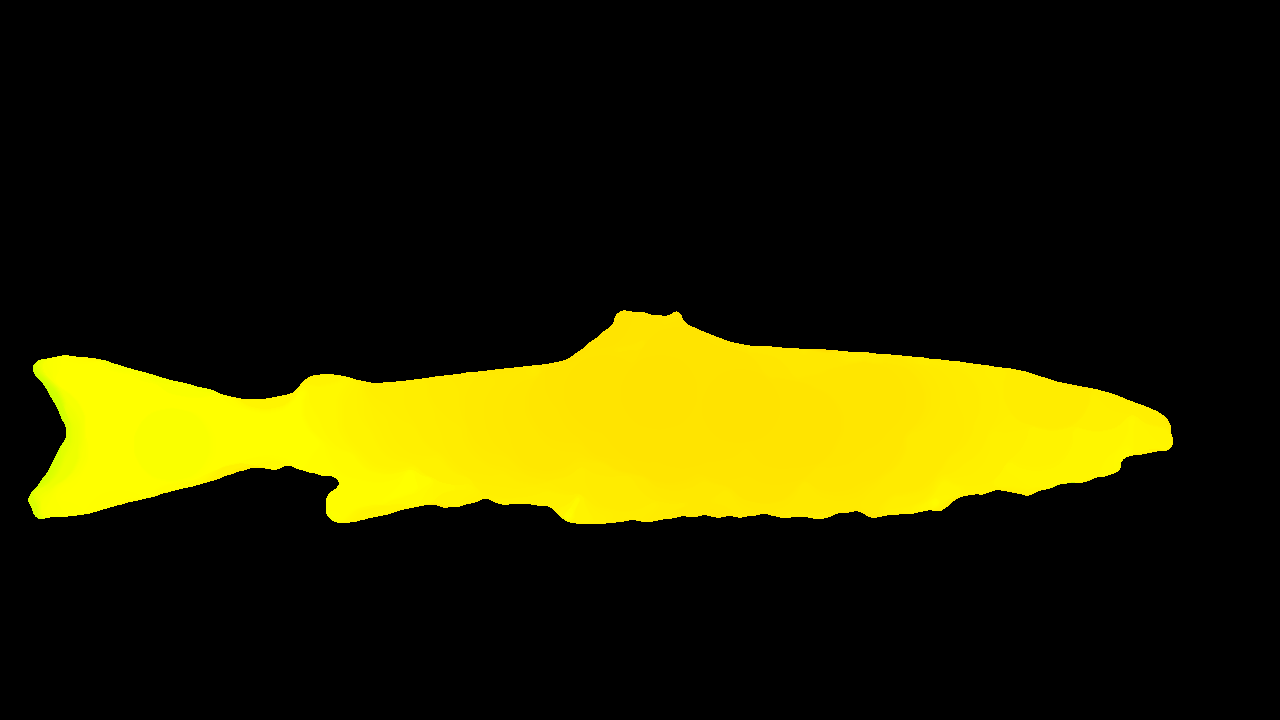
\includegraphics[width=\linewidth]{images/implementation/algorithm_test/median_filter_63}
        \caption{Result} 
        \label{fig:result_73}
    \end{subfigure}
    
    \medskip
    \begin{subfigure}{0.48\textwidth}
        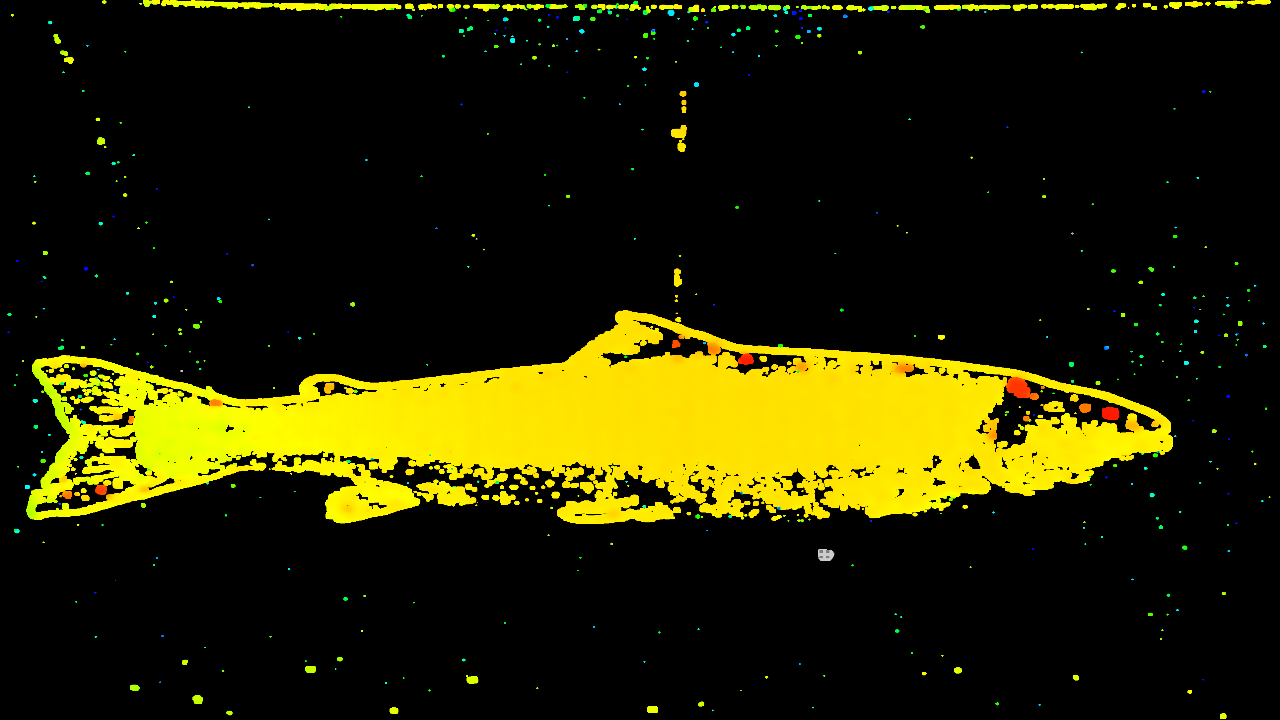
\includegraphics[width=\linewidth]{images/implementation/algorithm_test/original_82}
        \caption{Original depthmap image} 
        \label{fig:original_depthmap_82}
    \end{subfigure}\hspace*{\fill}
    \begin{subfigure}{0.48\textwidth}
        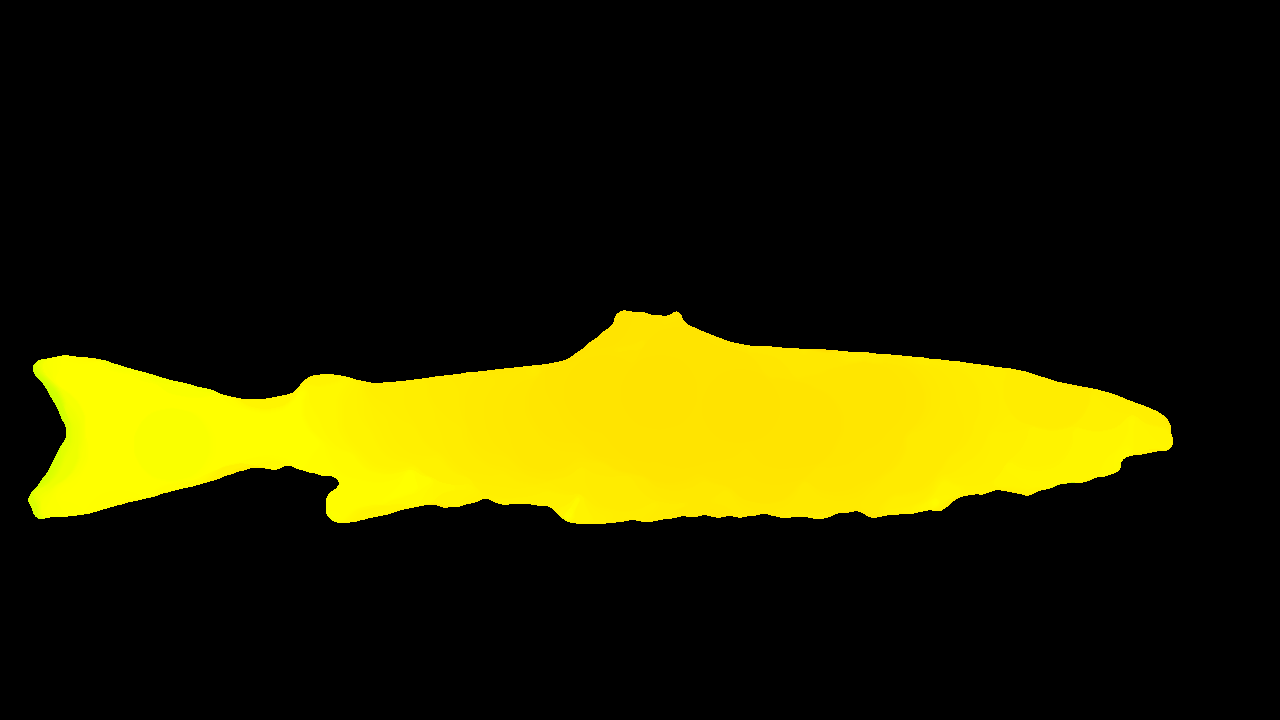
\includegraphics[width=\linewidth]{images/implementation/algorithm_test/median_filter_63}
        \caption{Result} 
        \label{fig:result_82}
    \end{subfigure}
    
    \medskip
    \begin{subfigure}{0.48\textwidth}
        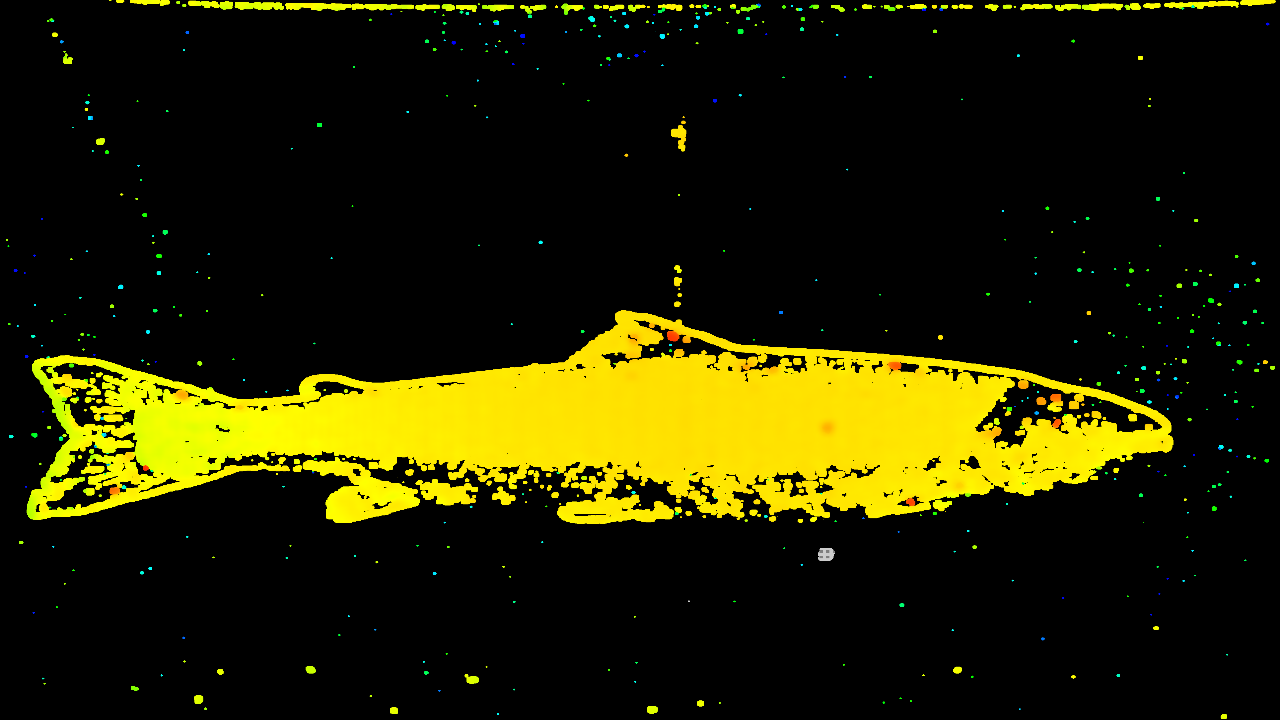
\includegraphics[width=\linewidth]{images/implementation/algorithm_test/original_87}
        \caption{Original depthmap image} 
        \label{fig:original_depthmap_87}
    \end{subfigure}\hspace*{\fill}
    \begin{subfigure}{0.48\textwidth}
        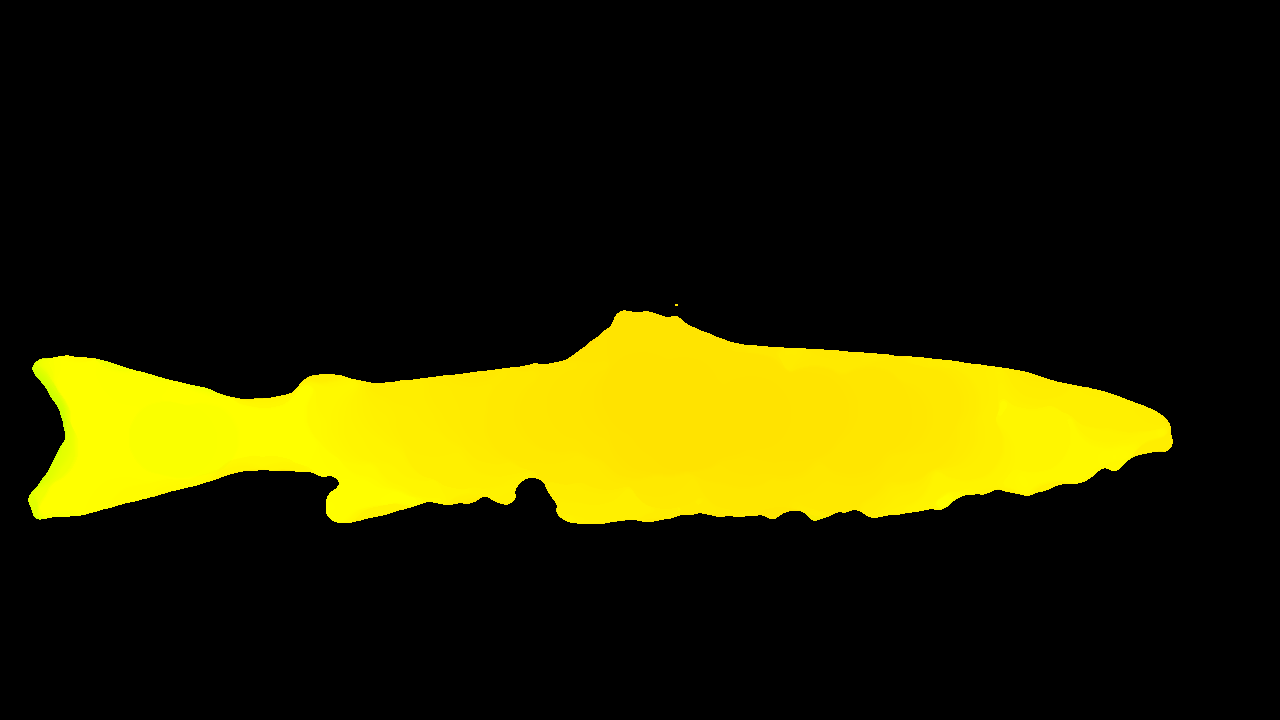
\includegraphics[width=\linewidth]{images/implementation/algorithm_test/median_filter_87}
        \caption{Result} 
        \label{fig:result_87}
    \end{subfigure}
    
    \caption{Algorithm test on different images} 
    \label{fig:algorithm_test}
\end{figure}

\newpage


%%%%%%%%%%%%%%%%%%%%%%%%%%%%%%%%%%%%%%%%%%%%%%%%%%%%%%%%%%%%%%%%%%%%%%


\subsection{Different Levels of Particle Noise}

To make the algorithm suitable for different conditions of water, noise was added to the depthmap.
The original plan was for the water to get blurry by it self since the dead salmons rotting process is very quick. The water, at the end of picture taking, looked very blurry and filled with particles, but it did not show much differences in the depthmap image. It's not known if it is mostly the water mediums properties that causes noise in the depthmap, and that particles are not enlarging this disorder significantly, or if enough particles within reason will disturb the depth measurements done by the Raytrix.

Since we could not get the naturally disturbances in the water to affect the depthmap directly, noise was added to the computed depthmap images.

The noise used is random sized color circles with random color placed randomly. The radius of each pixel is between 1 and 6 pixels. Noise was added from level 1 to 40, where level 1 starts with 20 particles, and each level adds 40 particles. That is, level 40 has 1,580 random particles in the image.

The algorithm has few problems up to level 20. Figure \ref{fig:noise_level_1}, and figure \ref{fig:noise_level_8} shows noise level 1 and 8, respectively, and shows few differences. After level 20, small parts of the fish starts missing (figure \ref{fig:noise_level_22}), and those holes get bigger and more concentrated up to level 40. Still, the algorithm can sometimes get decent results, an example is figure \ref{fig:noise_level_32}. Level 40 is almost covered with particles, and this would most likely never be a real issue, but the result is still not too bad.

If this technology is to be used in conditions containing more particles than from the test case used in this report, it is reasonable to believe that some more processing and tuning could give good results also then. The case would most likely be to fill in the missing parts even more, and perhaps calculate the largest contour from the totalfocus image instead of the depthmap. 





{\color{red} Put this in result???

It is seen from the noisy images that it has almost no effect on the result. This shows that the algorithm is robust and will work in most particle conditions as long as the light settings remains the same and the distance to the fish is within some boundaries. }


% NEW TEST

\begin{figure}[h]
    \centering
    \begin{subfigure}{1\textwidth}
        \centering
        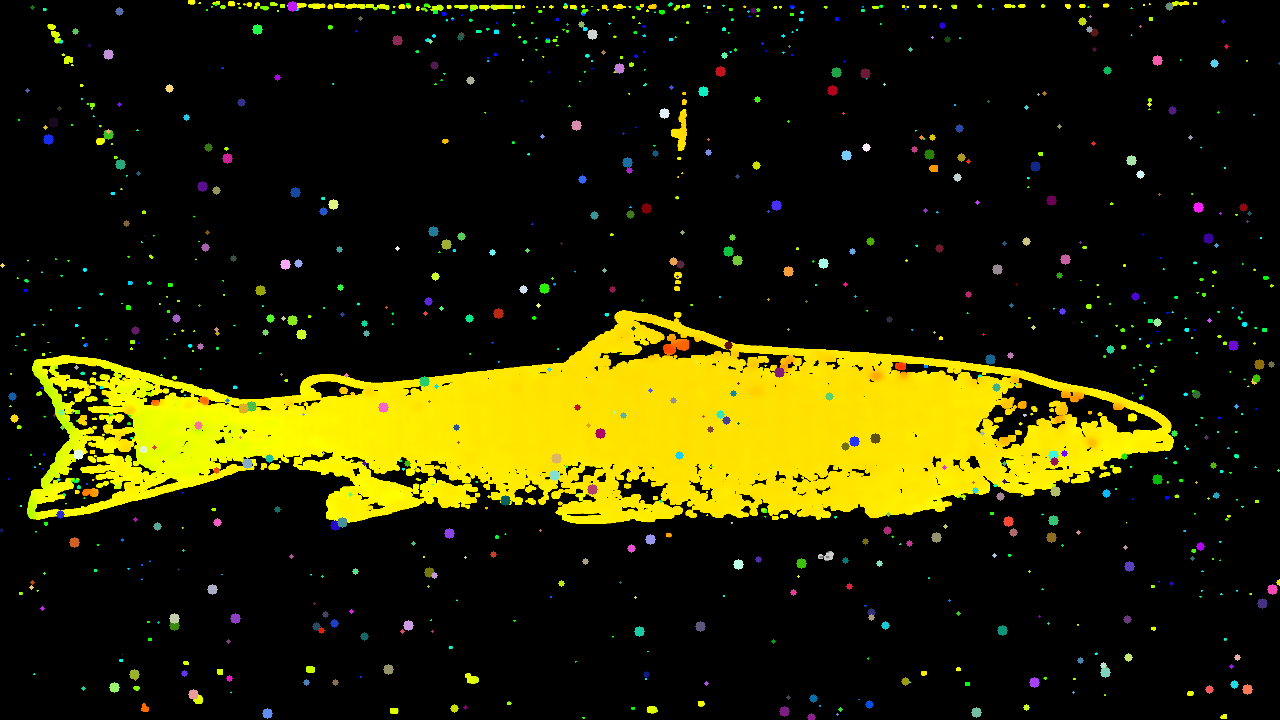
\includegraphics[width=.7\linewidth]{images/implementation/noise/noise63_1}
        \caption{Depthmap image with noise level 1} 
        \label{fig:image_noise_level_1}
    \end{subfigure}\hspace*{\fill}
    
    \medskip
    \begin{subfigure}{1\textwidth}
        \centering
        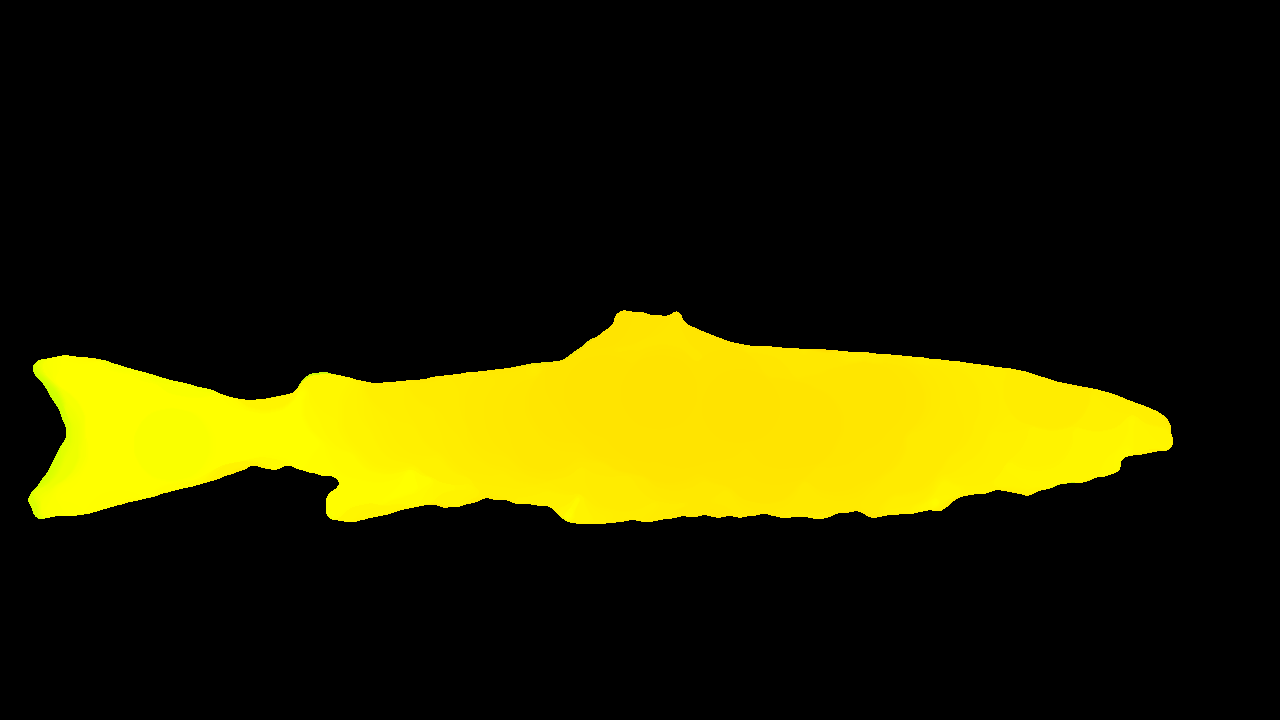
\includegraphics[width=.7\linewidth]{images/implementation/noise/filternoise63_1}
        \caption{Resulting depthmap} 
        \label{fig:filter_noise_level_1}
    \end{subfigure}\hspace*{\fill}
    \caption{Depthmap image and result for noise level 1}
    \label{fig:noise_level_1}
\end{figure}

\begin{figure}[h]
    \centering
    \begin{subfigure}{1\textwidth}
        \centering
        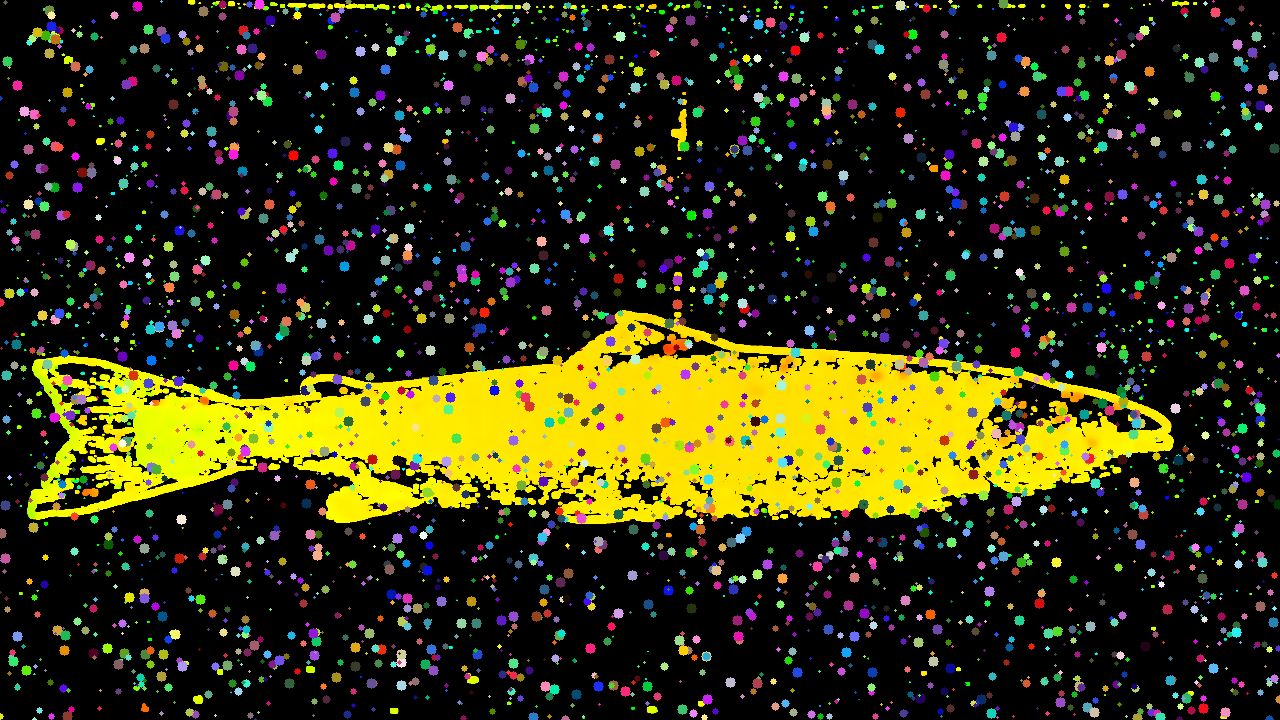
\includegraphics[width=.7\linewidth]{images/implementation/noise/noise63_8}
        \caption{Depthmap image with noise level 8} 
        \label{fig:image_noise_level_8}
    \end{subfigure}\hspace*{\fill}
    
    \medskip
    \begin{subfigure}{1\textwidth}
        \centering
        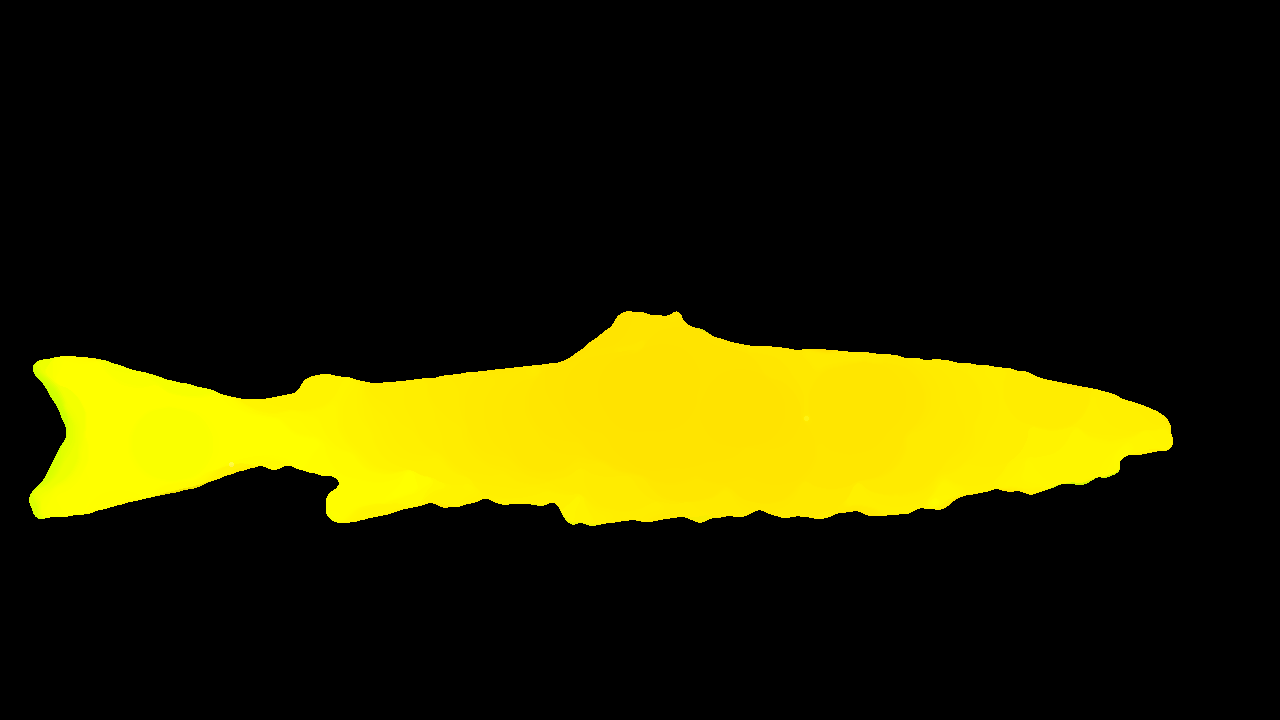
\includegraphics[width=.7\linewidth]{images/implementation/noise/filternoise63_8}
        \caption{Resulting depthmap} 
        \label{fig:filter_noise_level_8}
    \end{subfigure}\hspace*{\fill}
    \caption{Depthmap image and result for noise level 8}
    \label{fig:noise_level_8}
\end{figure}

\begin{figure}[h]
    \centering
    \begin{subfigure}{1\textwidth}
        \centering
        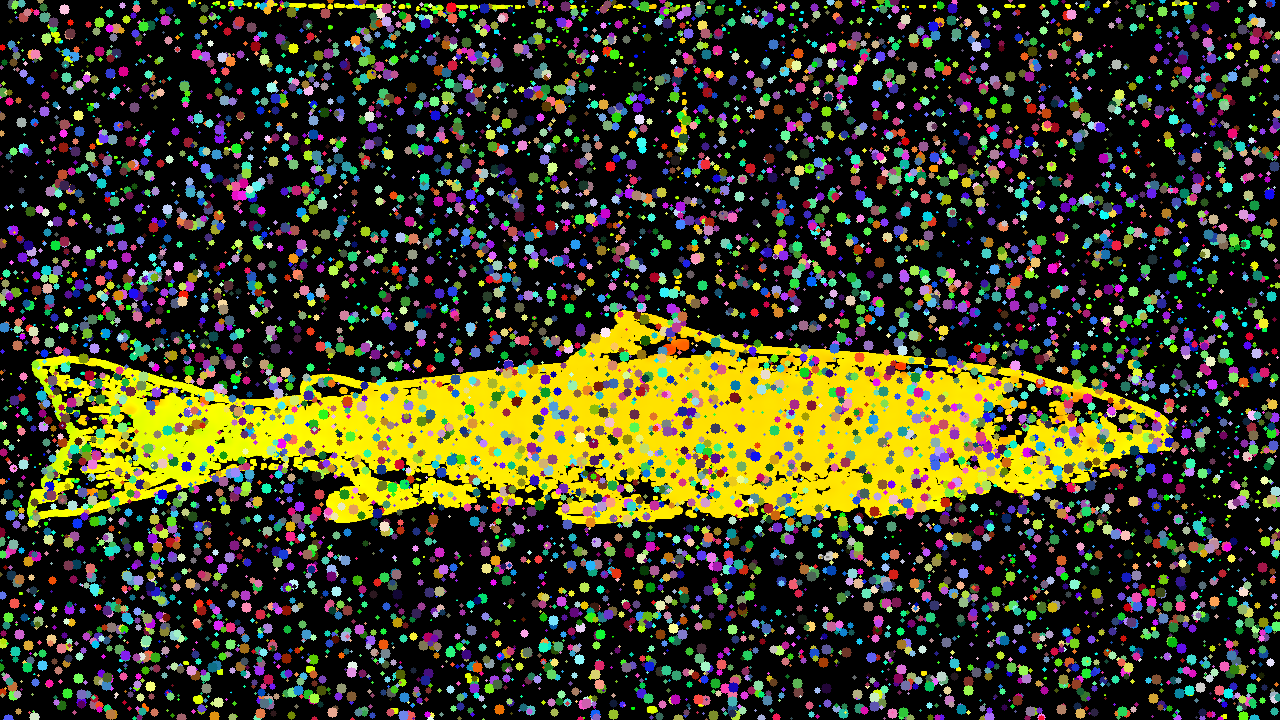
\includegraphics[width=.7\linewidth]{images/implementation/noise/noise63_22}
        \caption{Depthmap image with noise level 22} 
        \label{fig:image_noise_level_22}
    \end{subfigure}\hspace*{\fill}
    
    \medskip
    \begin{subfigure}{1\textwidth}
        \centering
        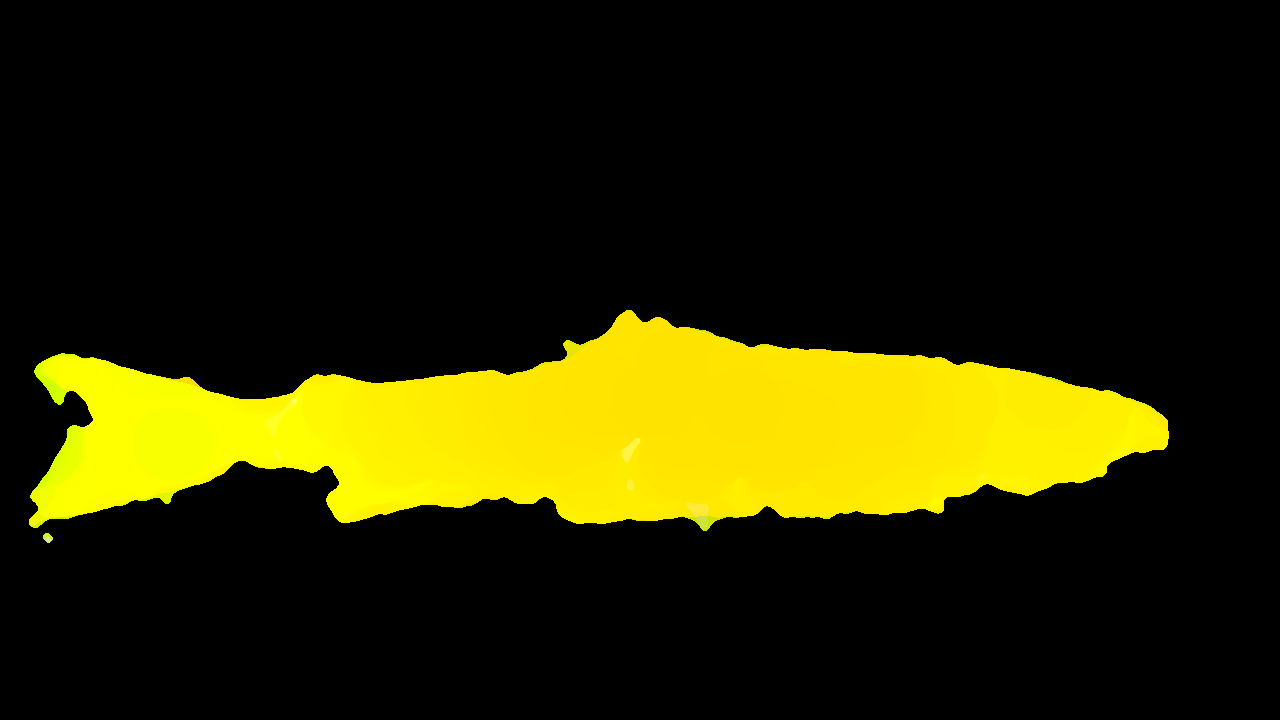
\includegraphics[width=.7\linewidth]{images/implementation/noise/filternoise63_22}
        \caption{Resulting depthmap} 
        \label{fig:filter_noise_level_22}
    \end{subfigure}\hspace*{\fill}
    \caption{Depthmap image and result for noise level 22}
    \label{fig:noise_level_22}
\end{figure}

\begin{figure}[h]
    \centering
    \begin{subfigure}{1\textwidth}
        \centering
        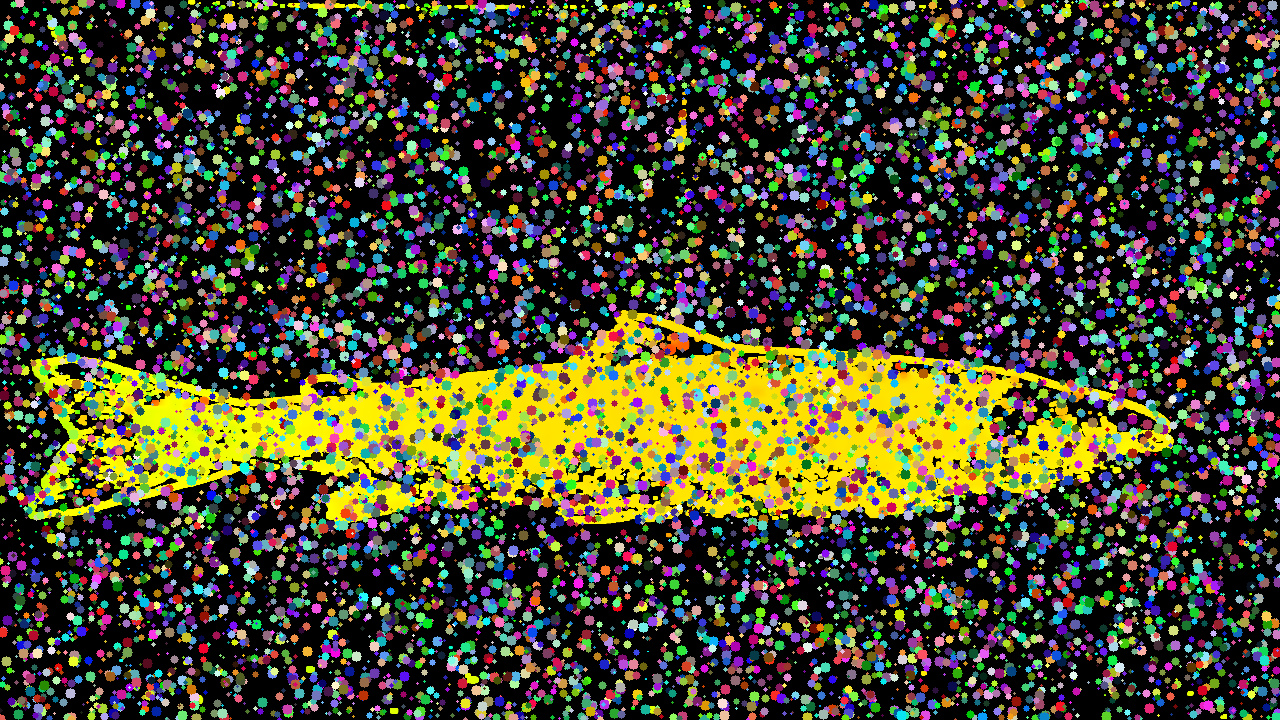
\includegraphics[width=.7\linewidth]{images/implementation/noise/noise63_32}
        \caption{Depthmap image with noise level 32} 
        \label{fig:image_noise_level_32}
    \end{subfigure}\hspace*{\fill}
    
    \medskip
    \begin{subfigure}{1\textwidth}
        \centering
        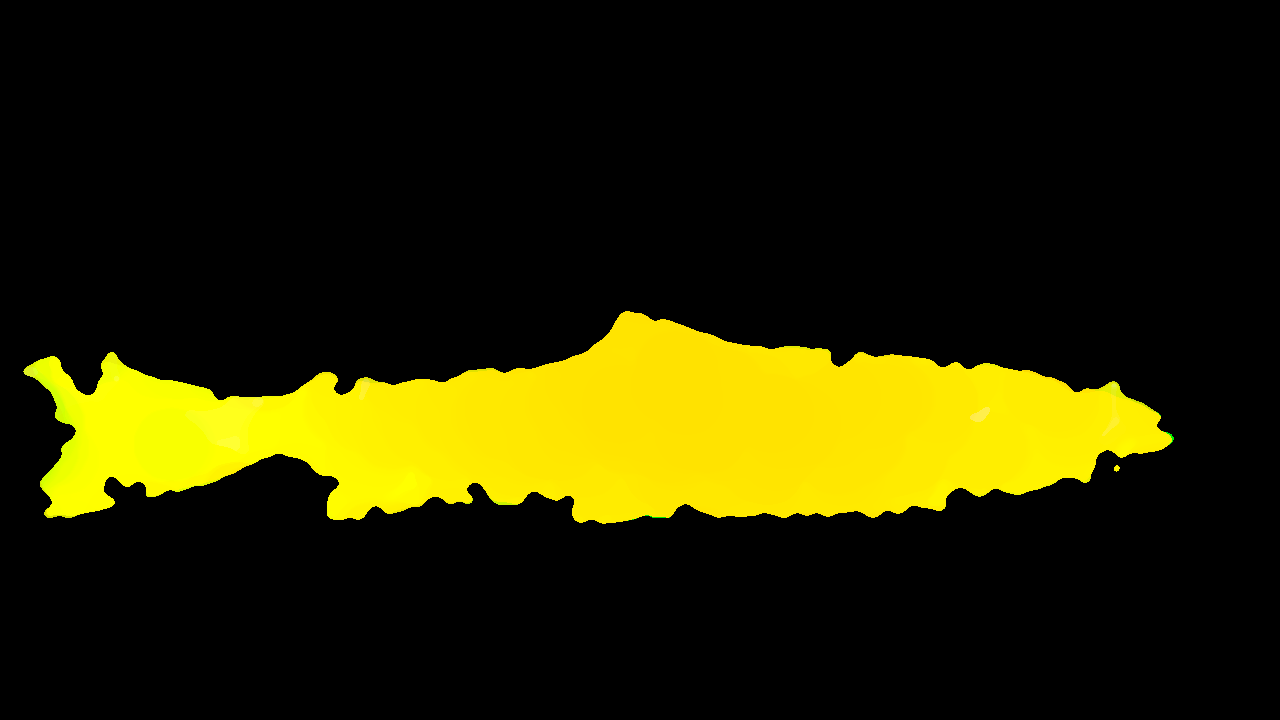
\includegraphics[width=.7\linewidth]{images/implementation/noise/filternoise63_32}
        \caption{Resulting depthmap} 
        \label{fig:filter_noise_level_32}
    \end{subfigure}\hspace*{\fill}
    \caption{Depthmap image and result for noise level 32}
    \label{fig:noise_level_32}
\end{figure}

\begin{figure}[h]
    \centering
    \begin{subfigure}{1\textwidth}
        \centering
        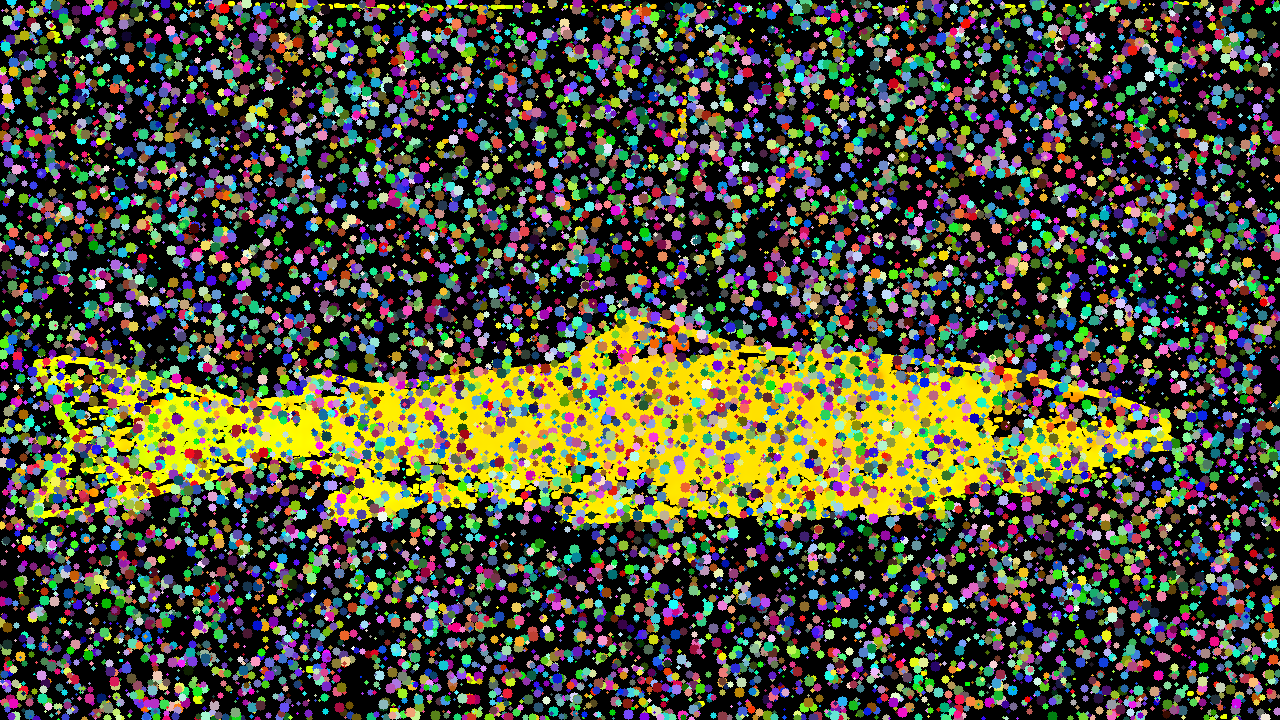
\includegraphics[width=.7\linewidth]{images/implementation/noise/noise63_40}
        \caption{Depthmap image with noise level 40} 
        \label{fig:image_noise_level_40}
    \end{subfigure}\hspace*{\fill}
    
    \medskip
    \begin{subfigure}{1\textwidth}
        \centering
        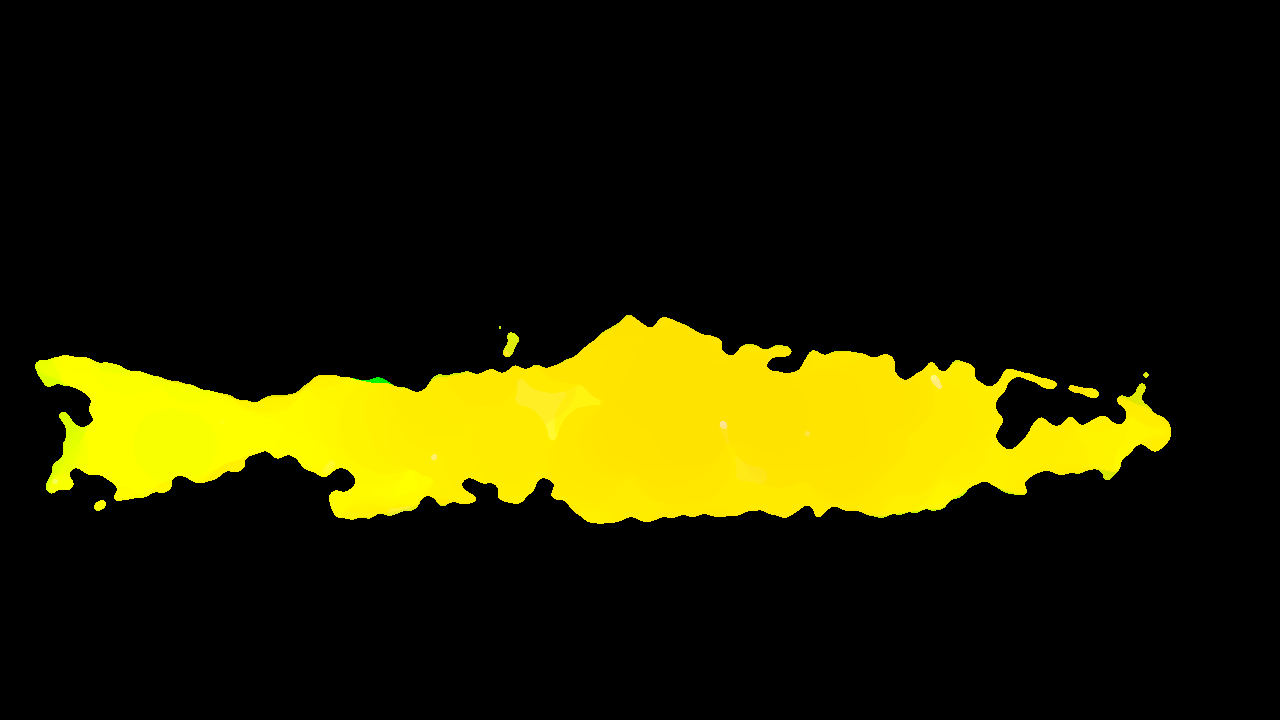
\includegraphics[width=.7\linewidth]{images/implementation/noise/filternoise63_40}
        \caption{Resulting depthmap} 
        \label{fig:filter_noise_level_40}
    \end{subfigure}\hspace*{\fill}
    \caption{Depthmap image and result for noise level 40}
    \label{fig:noise_level_40}
\end{figure}
